\section{Case Study}
\label{sec:case_study}

In this section, we provide a case study of magnetic control of
3-D plasma instabilities using the HBT-EP Tokamak equipped with
the GPU and the aforementioned I/O processing schemes.
This control system requires low latency and high computing capabilities
to achieve a sampling period of the order of ten microseconds, while
processing 96 inputs and 64 outputs of 16-bit data with a complex
algorithm.
Implementing the algorithm on the CPU failed due to insufficient real-time
performance. The case study presented herein, therefore, is significant in that we look
into a possibility of GPU implementations for the plasma control system.

\begin{figure}[t]
 \centering
 \includegraphics[width=\hsize]{eps/tokamak_sysarch.eps}
 \caption{HBT-EP magnetic sensors and control coils connected with the
 GPU.}
 \label{fig:tokamak_sysarch}
\end{figure}

Figure~\ref{fig:tokamak_sysarch} shows a system architecture used in
this case study.
The control input comes from a set of magnetic sensors through a D-TACQ
ACQ196 digitizer, and the resulting control signal is sent to two D-TACQ
AO32 analog output modules to excite control coils.
These input and output modules are connected to the NVIDIA GTX 580 upon the PCIe bus.
We evaluate three schemes against this system architecture
from the viewpoint of GPU execution costs for the control algorithm and
data I/O costs for the data transfer.
Each scheme is applied as follows:
\begin{itemize} \itemsep1pt
 \item In the {\hd} scheme, the device driver of the digitizer transfers
       the input data set to the buffers allocated on the host memory.
       The control program copies this data set to the device memory via
       PCI-mapped host memory space, and the parallelized control
       algorithm runs on the GPU with the data on the device memory.
       Once the output data set is produced by the GPU, the control
       program copies it back to the host memory, and it is finally
       pulled by the device driver of the analog output modules.
       This is the traditional form of GPU computing.
 \item The {\hp} scheme pins the input and output buffers to PCI-mapped
       host memory space.
       Since the data set pushed and pulled by the device drivers of
       the I/O modules is directly accessible to the GPU, there is no
       need to perform data copies.
       However, this scheme must compromise the latency of data access
       imposed on the GPU when executing the control algorithm.
 \item Similarly to the {\hp} scheme, the {\dm} scheme presented in this
       paper uses pinned PCI-mapped host memory space to allocate the
       input and out buffers, and further maps it to the device memory
       through PCI BAR space.
       Thus, there is no need of data copies while the data access of
       the control algorithm is limited within the device memory.
\end{itemize}

This paper does not provide the details of the control
algorithm which is outside the scope of this paper.
The outline of the control system implementation is that the host
program launches the device program on the GPU once at the beginning
when the system is loaded.
The device program polls until the input data set arrives.
This is due to a requirement of low-latency computing.
The input and output modules are configured to write the input data to
and read the output data from the specified PCI regions through DMA,
respectively.
These PCI regions are directly mapped to the device memory space
allocated by the control system, using the {\dm} scheme presented in this
paper.
In consequence, once the input and output modules are configured, and
the device program is launched at the beginning, the algorithm can keep
executing on the GPU, without accessing the CPU and the host memory at
all.

\begin{figure}[t]
 \centering
 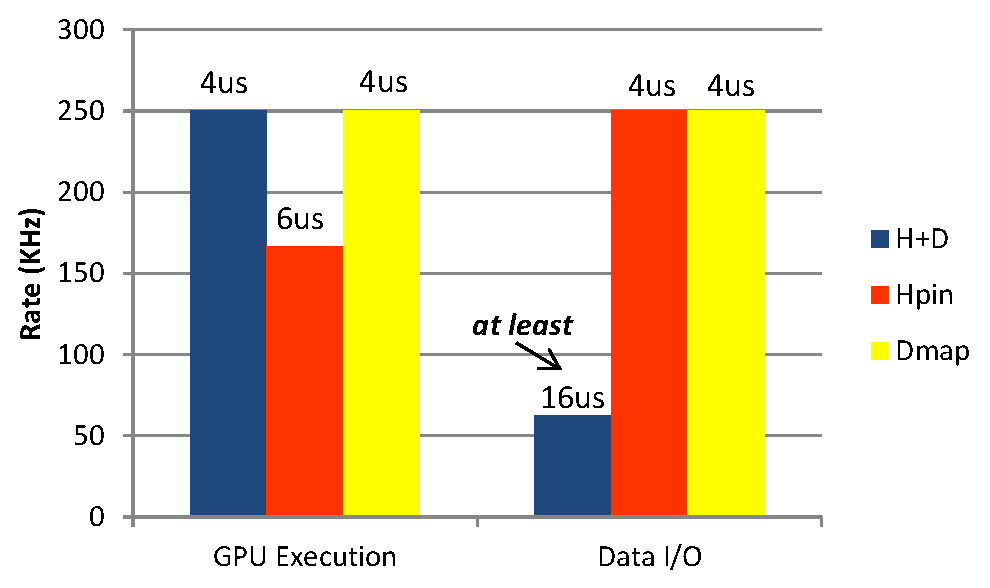
\includegraphics[width=\hsize]{eps/eval_plasma2.eps}
 \caption{\textit{Estimated} GPU execution and data I/O costs of
 the plasma control system.}
 \label{fig:eval_plasma}
\end{figure}

We now show that the {\dm} scheme reduces both GPU execution costs
for the control algorithm and data I/O costs for the data transfer.
Figure~\ref{fig:eval_plasma} shows the result of experiments conducted
under the three different schemes, respectively.
Note that the values of the GPU execution and the data I/O costs are
\textit{estimations}.
In the experiment, we could measure the sampling periods of the plasma
control system achieved the {\dm} and the {\hp} schemes while there was
no point of implementing the {\hd} scheme in terms of the total latency.
We could also measure the round-trip time of the data transfer between
the sensor/actuator and the GPU.
We estimate details of the GPU execution and the data I/O costs based on
these measured results.
In particular, our assumption is that the {\dm} and the {\hd} schemes
should have the same algorithm cycle, while the the {\dm} and the {\hp}
schemes should have the same data latency, by nature.
The {\dm} scheme achieves the highest rate in both algorithm
execution and data transfer.
The remaining two schemes, on the other hand, compromise one or the
other of them.
The {\hd} and the {\dm} schemes exhibit the same performance level for
algorithm execution since they both use the device memory, while the
data transfer latency of the {\hp} and the {\dm} schemes are equivalent
since they both remove data copies.
Comparing the {\hd} and the {\hp} schemes, one can also see that the
impact of overhead introduced by data copies, \textit{i.e.}, $16\mu$s, is
greater than that introduced by the GPU accessing pinned host memory
space, \textit{i.e.}, $6\mu$s, on the overall system performance.
Curiously, there is additional latency of $4\mu$s observed when running
the control system.
We suspect that this latency comes from some interactions among the host
computer, the graphics card, and the I/O modules.
Lessons learned from this evaluation are summarized as follows:
\begin{itemize} \itemsep1pt
 \item Zero-copy I/O processing is very effective for this control
       system, reducing the latency of data transfer from $16\mu$s to
       $4\mu$s.
       The speed-up ratio is 4$\times$.
 \item Furthermore, the {\dm} scheme reduces the cycle time of algorithm
       execution from $6\mu$s to $4\mu$s.
       The speed-up ratio is 1.5$\times$.
       Since the HBT-EP Tokamak accommodates up to 216 inputs,
       meaning that the cycle time of algorithm execution is more
       dominated by data accesses, the benefit of the {\dm} scheme over
       the {\hp} scheme would be more significant for a larger scale of
       plasma control.
\end{itemize}

\begin{figure}[t]
 \centering
 \includegraphics[width=\hsize]{eps/oscilloscope.eps}
 \caption{Screenshot of the oscilloscope.}
 \label{fig:oscilloscope}
\end{figure}

The above measurement explains that the control system can operate at a
latency of $16\mu$s.
The data transfer from and to the input and output modules takes $4\mu$s
each.
The algorithm execution takes $4\mu$s.
Adding additional latency of $4\mu$s, the total control rate must be
able to achieve $16\mu$s.
Figure~\ref{fig:oscilloscope} depicts the screenshot of the oscilloscope
where we measure the signals of the input and the output modules.
The topmost and middle signals represent the input and the output,
respectively, while the lower signal indicates the base clock.
The grid spacing of the X axis is $5\mu$s.
The time interval from the first downward edge in the clock signal after
the input signal goes up to the instant when the output signal starts
uprising is almost equal to $16\mu$s.
This means that the total control processing time is $16\mu$s. 

We next demonstrate that the control system is running properly at a
rate of $16\mu$s.
The control input comes from a set of magnetic sensors arranged in a
ring, as illustrated in Figure~\ref{fig:tokamak_sysarch}, and the
magnetic field that they measure is rotating, whose orientation is
described by a \textit{phase}.
Ideally, the phase is equivalent to multiplication of time and
frequency.
To control this mode, the control system needs to produce a control
signal that generates an equal and opposite field, which also needs to
rotate.
Obviously, the two fields should have a constant phase difference,
because it is given by multiplication of the control processing time and
the rotation frequency.
However, in practice, the rotation frequency is not constant but is
changing.
As a result, the phase difference appears to oscillate, with the base
output signal, which can be found as spikes in
Figure~\ref{fig:phase_base}.
Now, we measure the phase difference with the output signal time-shifted
by $16\mu$s.
In other words, the effective control system latency is reduced by
$16\mu$s.
As shown in Figure~\ref{fig:phase_shifted}, the spikes are now all
removed.
This indicates that the control system is perfectly in phase with the
mode, and the effective control system latency now must be zero,
\textit{i.e.}, the actual latency is $16\mu$s.

\begin{figure}[t]
 \centering
 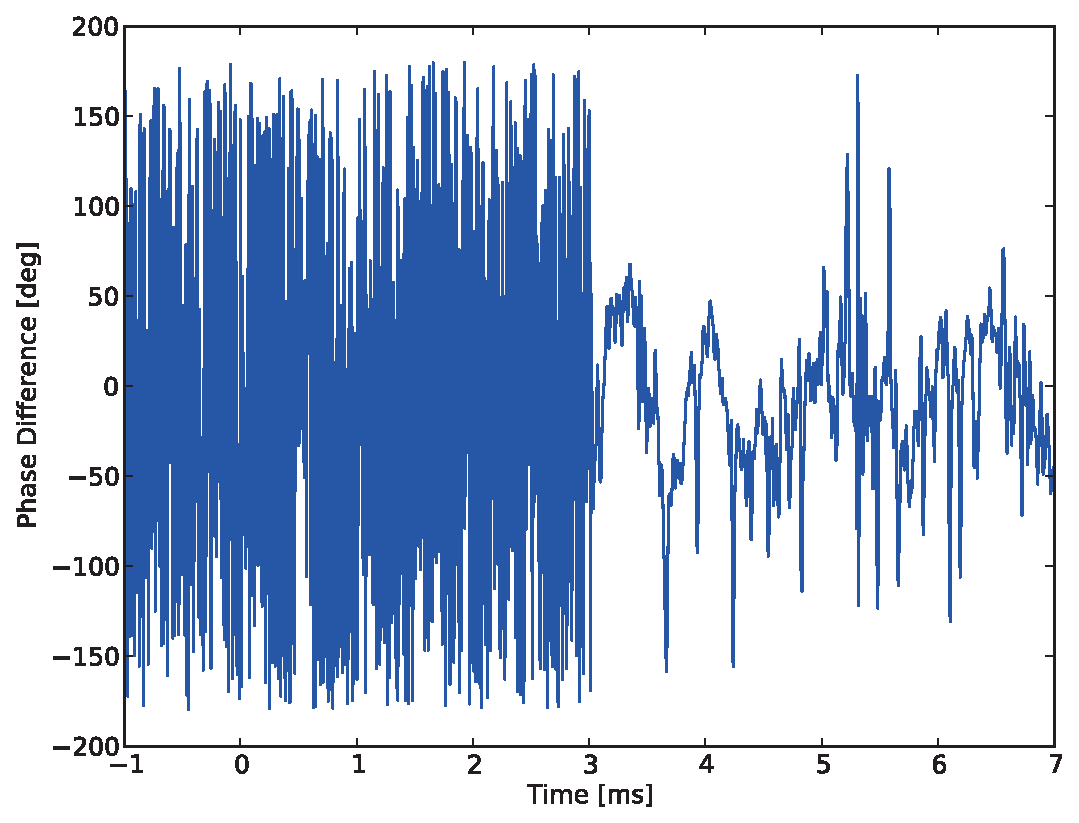
\includegraphics[width=\hsize]{eps/75221_base.eps}
 \caption{Phase difference observed with the base output signal.}
 \label{fig:phase_base}
\end{figure}
\begin{figure}[t]
 \centering
 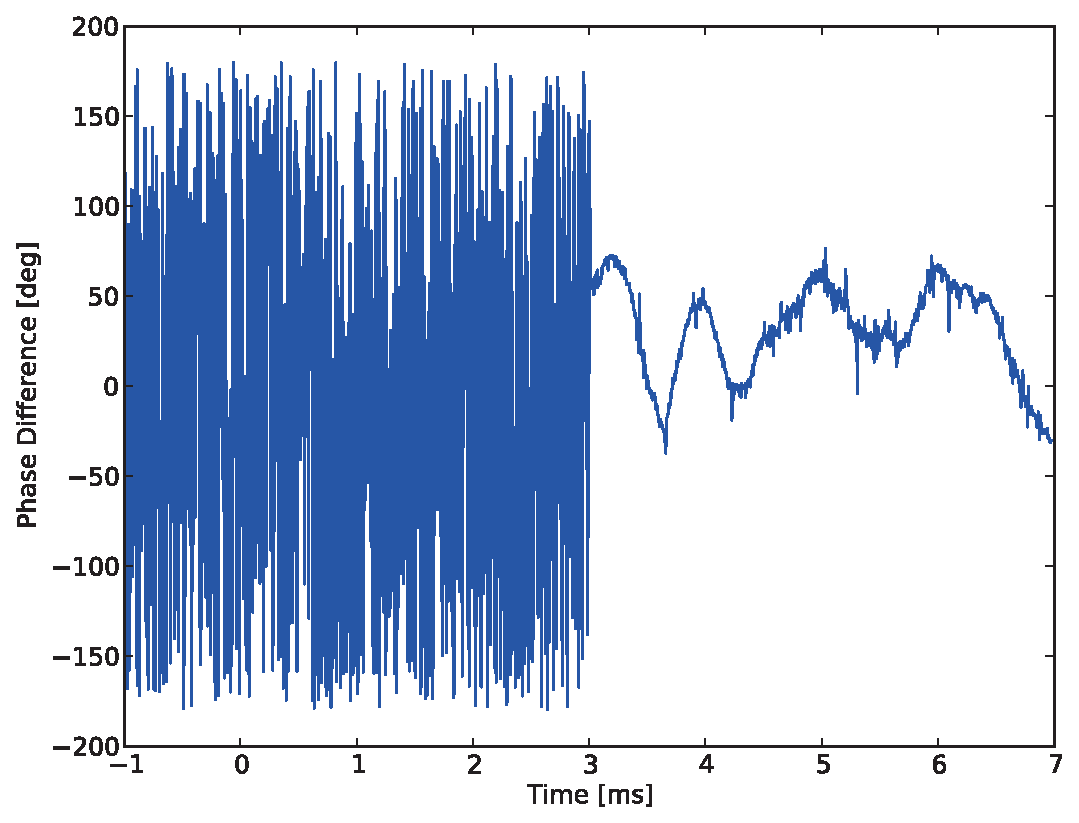
\includegraphics[width=\hsize]{eps/75221_shifted.eps}
 \caption{Phase difference observed with the output signal shifted by 16$\mu$s.}
 \label{fig:phase_shifted}
\end{figure}

\begin{figure}[t]
 \centering
 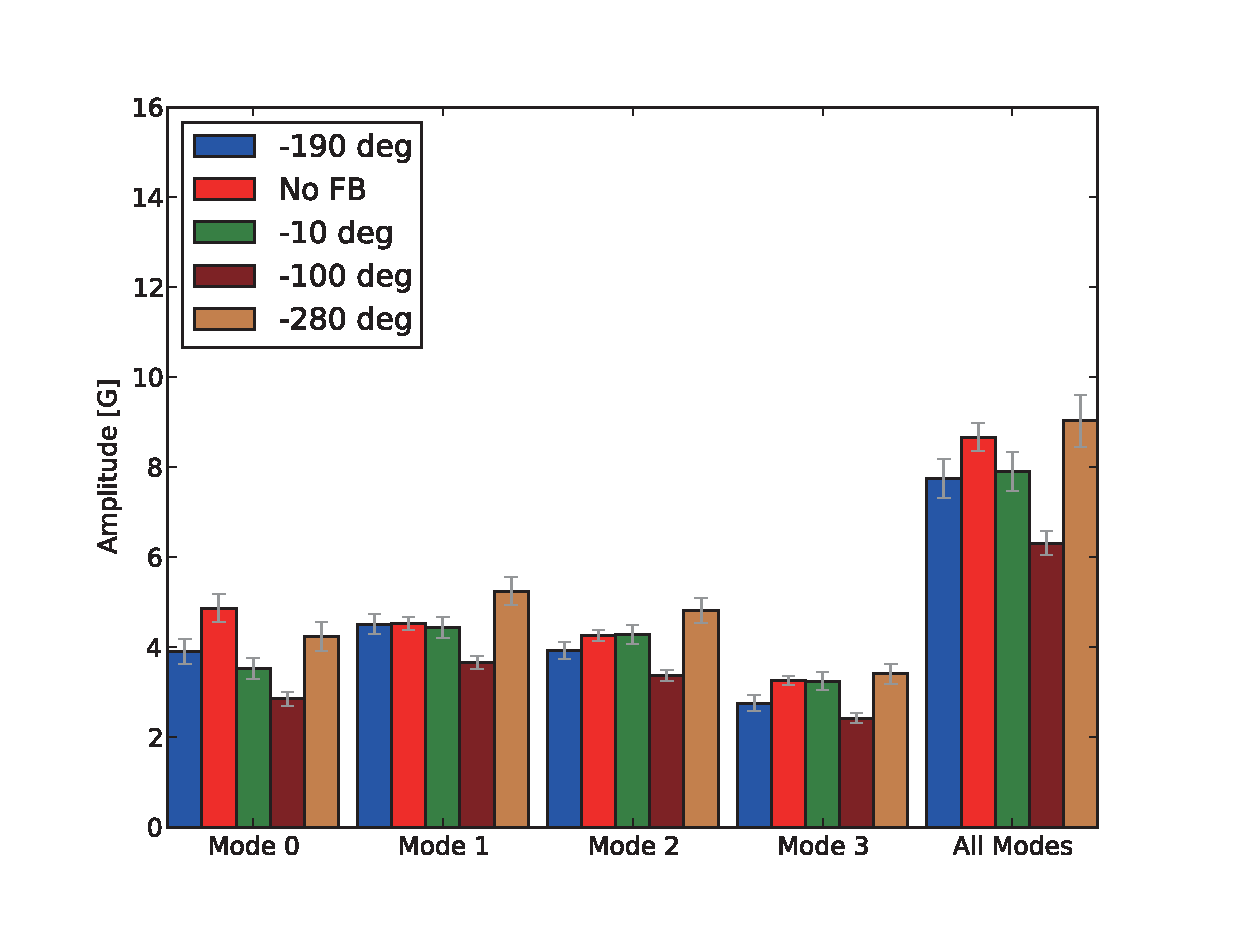
\includegraphics[width=\hsize]{eps/overview.eps}
 \caption{Practical findings of plasma control.}
 \label{fig:plasma_overview}
\end{figure}

Finally, we discuss practical findings of plasma control regarding the
HBT-EP ``Tokamak'' device.
Figure~\ref{fig:plasma_overview} shows a comparison of the average
perturbation amplitudes with different phasing.
The control system incorporates four arrays of magnetic sensors and
control coils, each of which controls one specific mode.
They are placed at different poloidal angles around the toroidal ring.
Due to their different locations, they measure slightly different
amplitudes.
From this experiment, we find that feedback at 280 degrees excites
perturbation, while feedback at 100 degrees is the right range for
suppression.
As compared to no feedback scenario (``No FB'' in the figure), for
example, we find that we can suppress the strength of the rotating field
by up to 30\% for any mode observed in this experiment.
